%****************************************************************
% Chapter X
%****************************************************************
\label{chapter-performance}
\chapter{Performance}

%****************************************************************
What is great about the Android runtime is that most of the stress of memory reclamation is done for developers. The system will track what developers are doing and when it sees that an object is not needed anymore, it will free it on their behalf. However, this does not exclude performance problems from happening here. When the amount of memory have allocated reaches an upper limit, a Garbage Collection (GC) event will be kicked off to free any resources that might not be needed any longer, freeing up space for future allocations. 

Anytime the frame drips about the $16$ milliseconds barrier, and the users are going to start to notice \ref{fig:16ms-per-frame}. So any code that forces allocated memory to spike above this threshold can cause problems. For instance, memory can become tighter, if the developer is allocating and freeing a large number of objects in a short period of time, the temporary objects again kicking off GC event. As result, increasing the risk of Memory leaks. They are objects which the application is no longer using, but the garbage collector fails to recognize them as unused.

\begin{figure}[H]
\caption{16ms Per Frame}
\label{fig:16ms-per-frame}
\centering
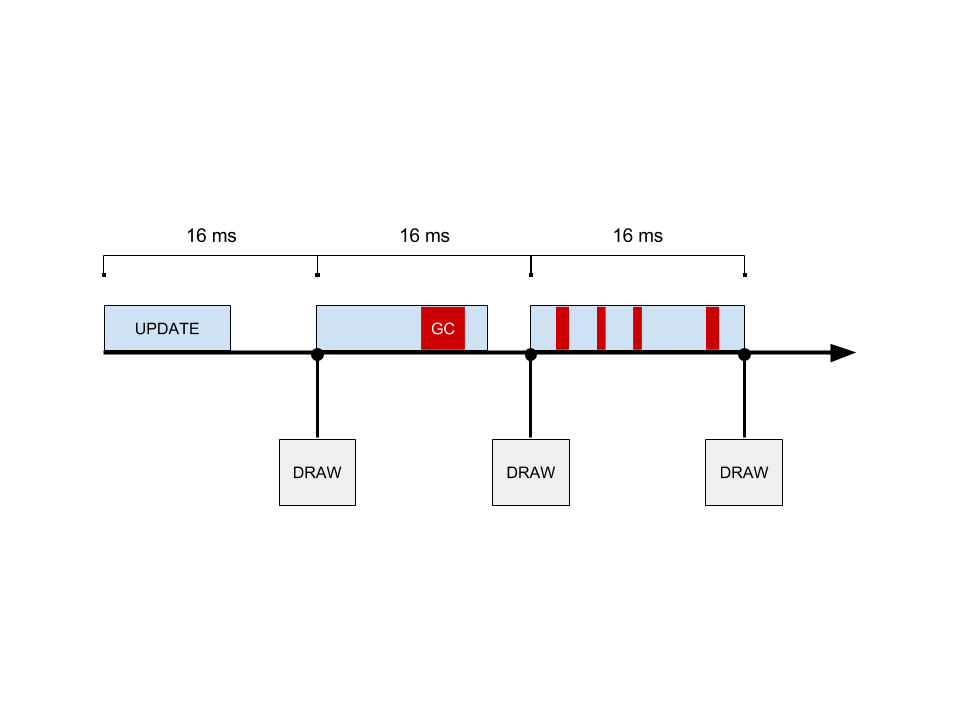
\includegraphics[width=\textwidth, keepaspectratio]{Figures/16ms-per-frame.png}
\decoRule
\end{figure}

Therefore, a performance testing is important for avoiding nasty GC events. Each GC event that developer can avoid, the application has more time per frame to do interesting things. In order to find out where in the code objects are being created but not released, created and not used, or created new when the developer could have been reusing them from existing objects. Android Studio provides a series of performance testing tools, such as Memory Monitor, Allocation Tracker, Heap Viewer, and the Systrace (it is an Android system trace tool helps developers analyze how the execution of the application fits into the many running systems on an Android device \cite{google.systrace.2016}).

In this case, according to the runtime, the performance analysis is divided into two parts: acyclic process and cyclic process. Task that required repeatedly executed during the render cyclicity of each frame is the factors influencing the runtime performance. In this chapter, the performance came from Android phone $Nexus 6P$.

%****************************************************************
\section{Acyclic}

%****************************************************************
In order to avoid UI being block, all of acyclic process in the application are handled in the new threads. In this section, I present the performance of geometric vertices' generation for \code{Placemark} (Icosphere) and \code{Earth} (UV Sphere) which only executes one time (or not) when needed. The geometric data for Icosphere generation will be cached once it has been created before. This is useful to avoid duplicate creations for same geometric vertices. The same cache solution for image and text data from \code{Placemark} description URL.

Based on the varying roundness of the Icosphere, it could evolve into a sphere has different vertex count \ref{tab:icosphere-level}. In general, level $3$ Icosphere is enough for illustrating a sphere, and in the application the \code{Placemark} is created on level $1$ Icosphere.

\begin{table}[H]
	\caption{Icosphere Level}
	\label{tab:icosphere-level}
	\centering
	\begin{tabular}{l l}
		\toprule
		\tabhead{Recursion Level} & \tabhead{Vertex Count}\\
		\midrule
		0 & 12\\
		1 & 42\\
		2 & 162\\
		3 & 642\\
		4 & 2562\\
		5 & 10242\\
		\bottomrule
	\end{tabular}
\end{table}

\begin{figure}[H]
	\caption{Icosphere performance}
	\label{fig:icosphere-performance}
	\centering
	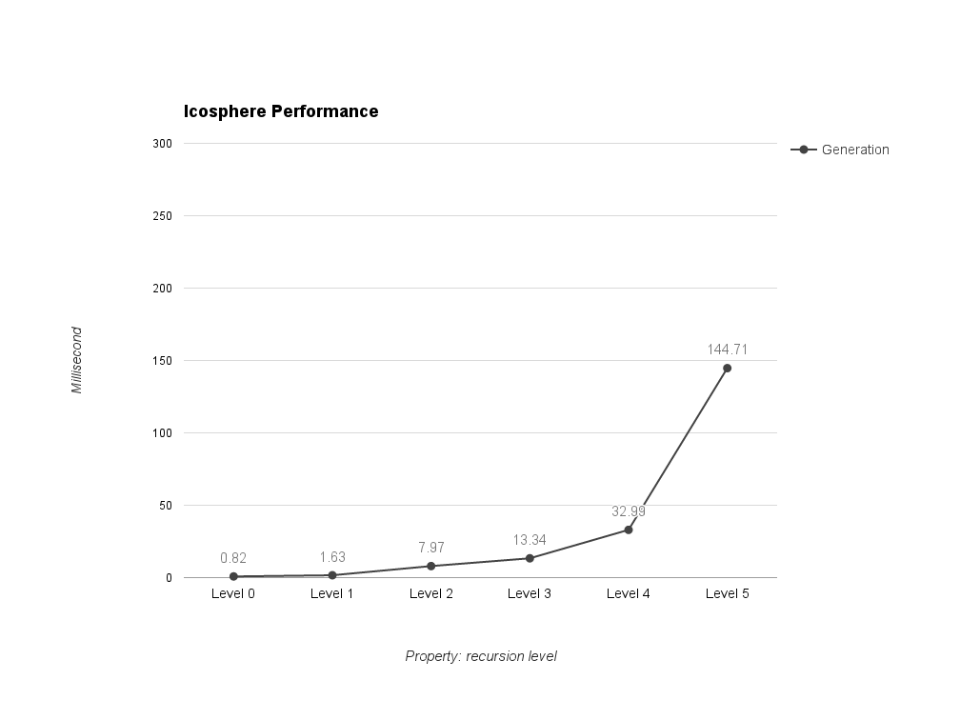
\includegraphics[width=\textwidth, keepaspectratio]{Figures/icosphere-performance.png}
	\decoRule
\end{figure}

The roundness of a UV Sphere depends on the partition level on both horizontal (ring) and vertical (segment) which denotes the axes of the 2D texture. The Earth is casually implemented as a $180 / 180$ UV Sphere in the application.

\begin{figure}[H]
	\caption{UV Sphere performance}
	\label{fig:uv-sphere-performance}
	\centering
	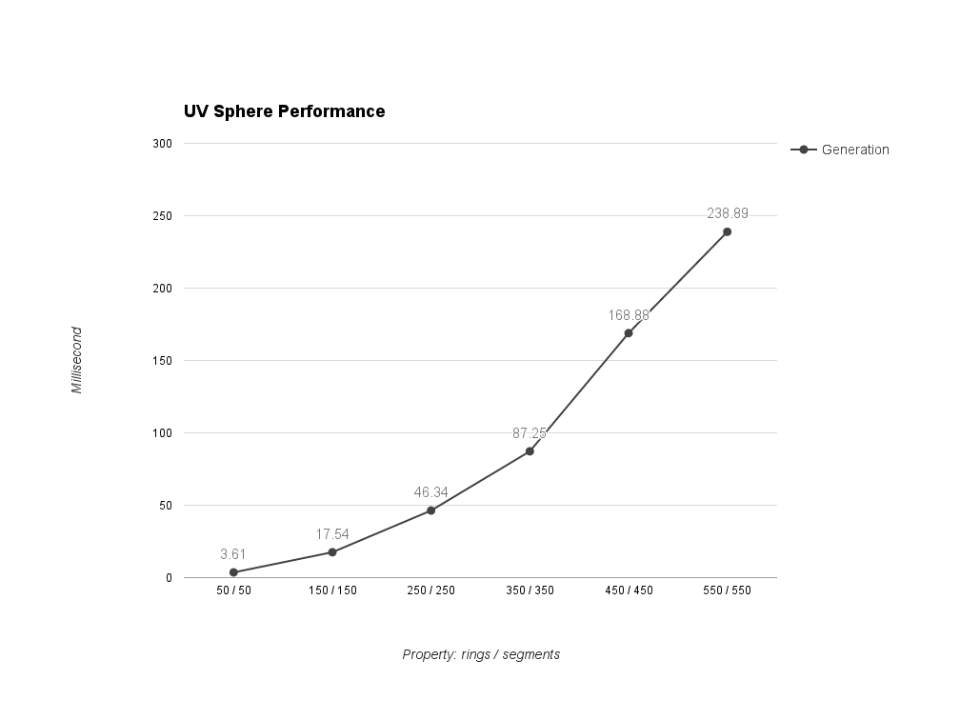
\includegraphics[width=\textwidth, keepaspectratio]{Figures/uv-sphere-performance.png}
	\decoRule
\end{figure}

Figure \ref{fig:geographic-data-performance} is the performance of initializing geographic data, including parsing KML files, transformation coordinate system from LLA to ECEF for each \code{Placemark}, etc.

\begin{figure}[H]
	\caption{Geographic Data Performance}
	\label{fig:geographic-data-performance}
	\centering
	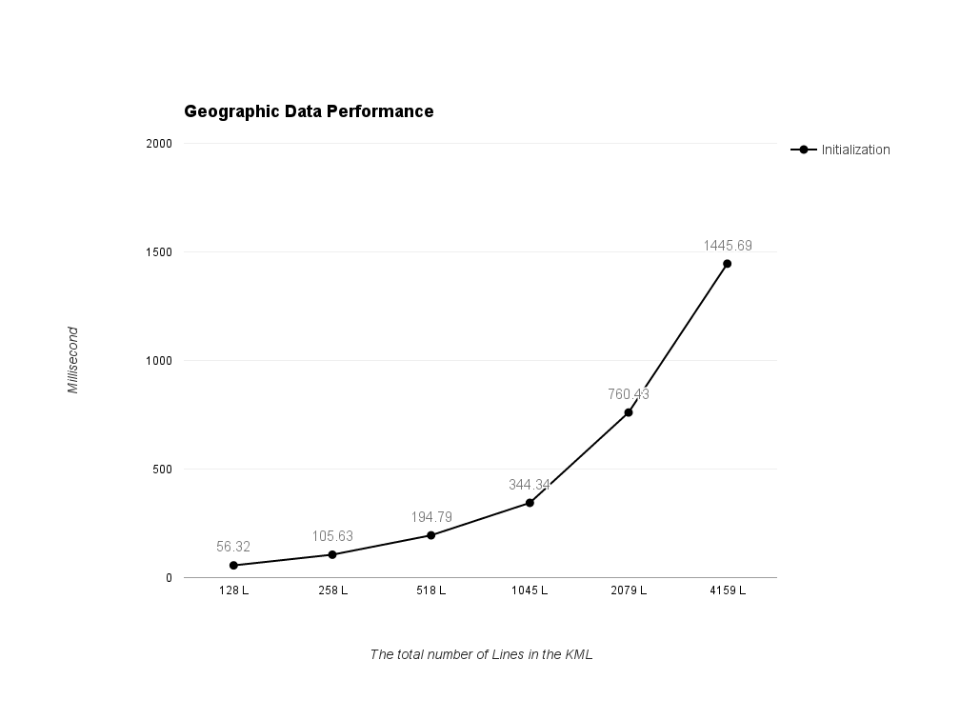
\includegraphics[width=\textwidth, keepaspectratio]{Figures/geographic-data-performance.png}
	\decoRule
\end{figure}

%****************************************************************
\section{Cyclic}

%****************************************************************



%The application has $55$ to $60$ FPS when the there is less than 250 \code{Placemark} exist in the scene. Although, the space partition that optimizes the intersection test has been significantly improved the performance. However, there is a performance limitation of current implementation due to the expensive render call in Android OpenGL ES API. It has a high priority and needs to be solved by calling the function once for all the same objects (\code{Placemark}).



%in a world where you app is not doing much of anything, you should see a flat graph  just like this one. From a performance perspective , this is actually an ideal scenarion. As you app allocates and free memory, you will see  the allocative amount fluctuate in your graph at the same time. any time you allocated memory drops by a significant amount, thats a signal that GC event has occurred. These GC events arenot  generally a noticeable performance problem, however a lots of them occurring over and over and over again in a short period of time can actually lead to performance issues. the more time you are spending doing GC, the less time you will have to do other stuff.



\begin{figure}[H]
	\caption{Memory Monitor}
	\label{fig:memory-monitor}
	\centering
	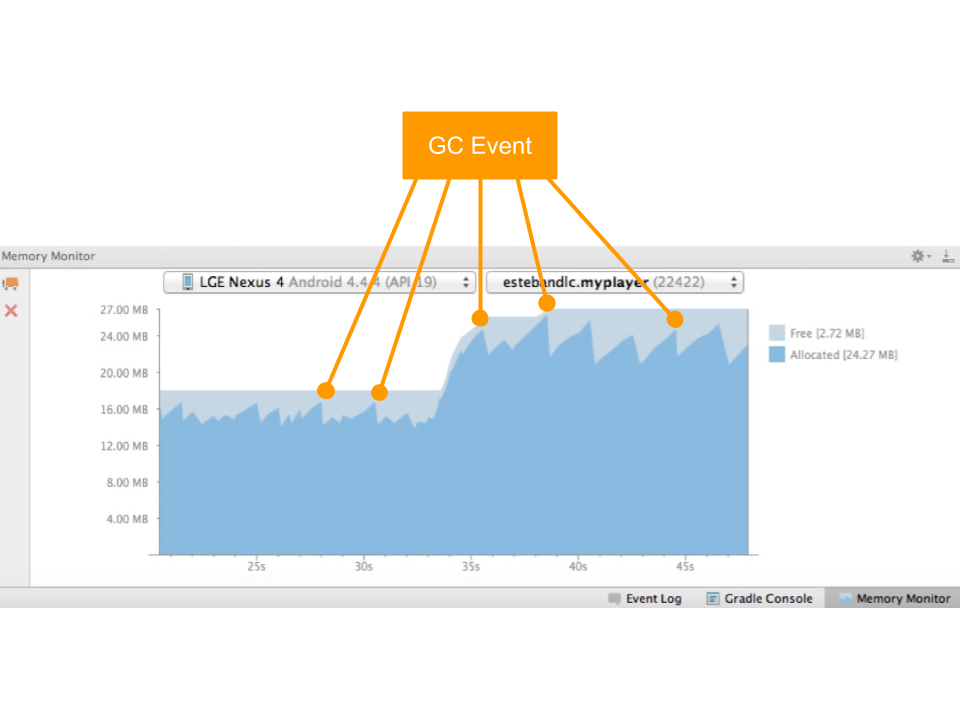
\includegraphics[width=\textwidth, keepaspectratio]{Figures/memory-monitor.png}
	\decoRule
\end{figure}



\begin{figure}[H]
	\caption{Memory Performance}
	\label{fig:memory-performance}
	\centering
	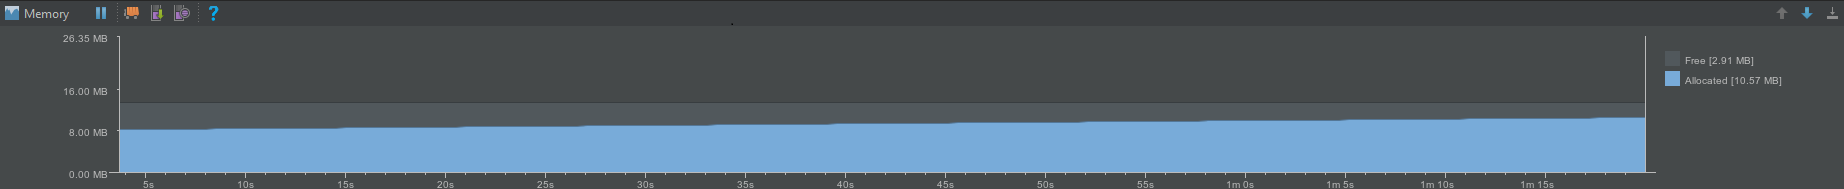
\includegraphics[width=\textwidth, keepaspectratio]{Figures/memory-performance.png}
	\decoRule
\end{figure}



\begin{figure}[H]
	\caption{Placemarks Intersection Performance}
	\label{fig:placemarks-intersection-performance}
	\centering
	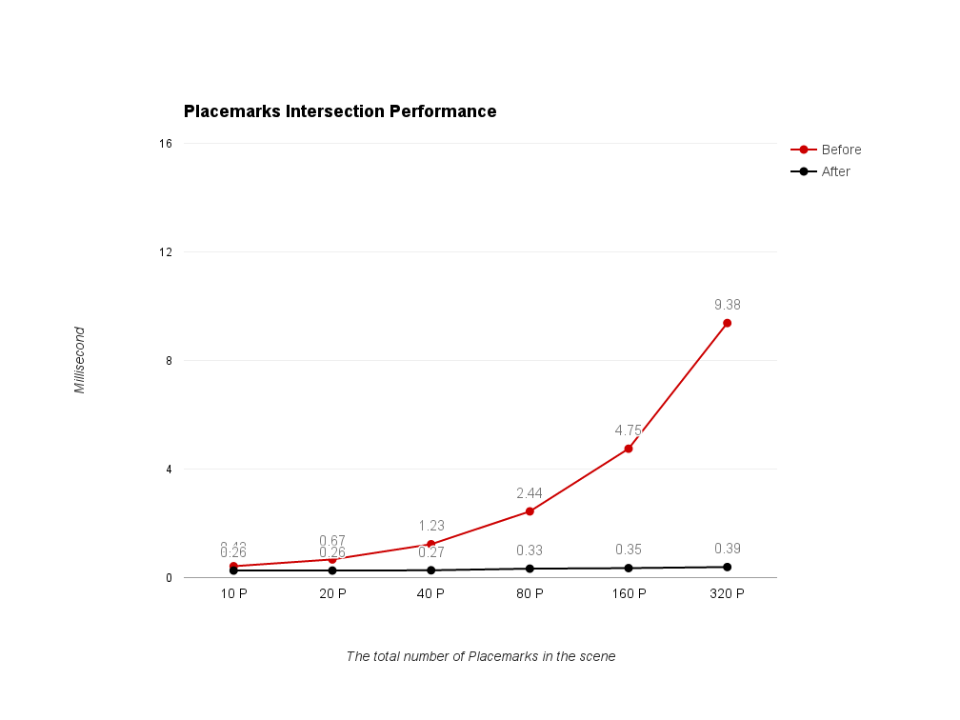
\includegraphics[width=\textwidth, keepaspectratio]{Figures/placemarks-intersection-performance.png}
	\decoRule
\end{figure}



\begin{figure}[H]
	\caption{Placemarks Update Performance}
	\label{fig:placemarks-update-performance}
	\centering
	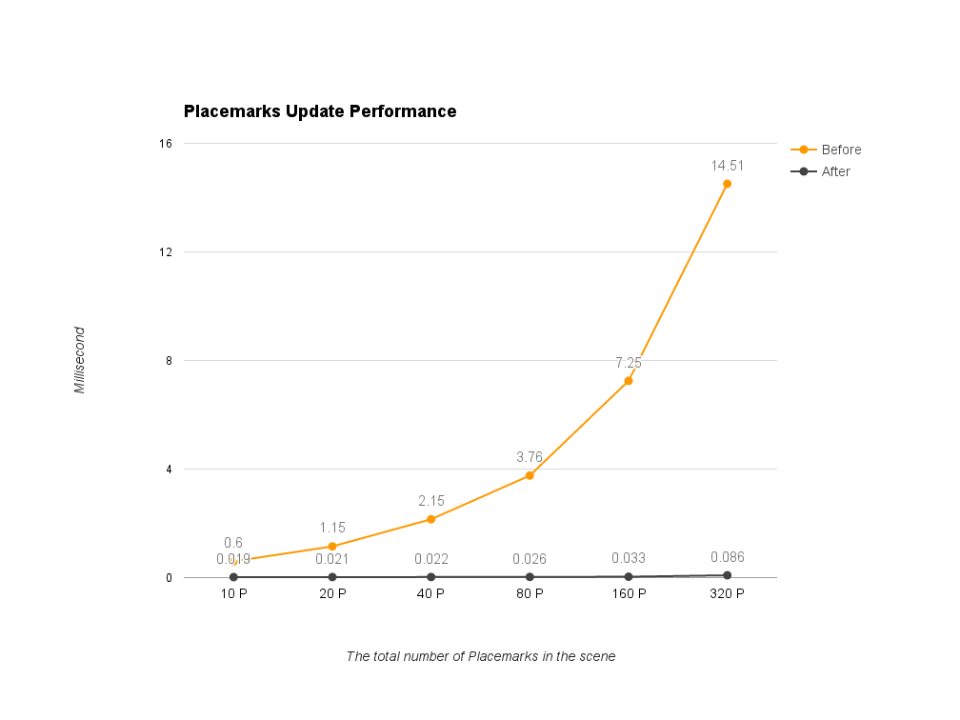
\includegraphics[width=\textwidth, keepaspectratio]{Figures/placemarks-update-performance.png}
	\decoRule
\end{figure}



\begin{figure}[H]
	\caption{Placemarks Draw Performance}
	\label{fig:placemarks-draw-performance}
	\centering
	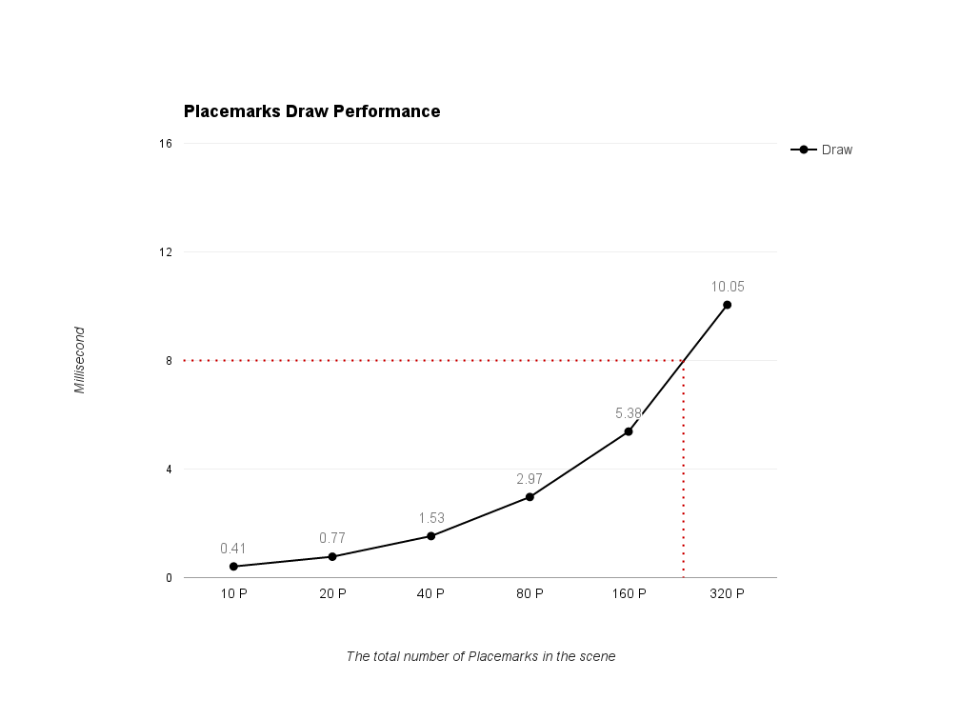
\includegraphics[width=\textwidth, keepaspectratio]{Figures/placemarks-draw-performance.png}
	\decoRule
\end{figure}



\begin{figure}[H]
	\caption{glDrawElements Performance}
	\label{fig:glDrawElements-performance}
	\centering
	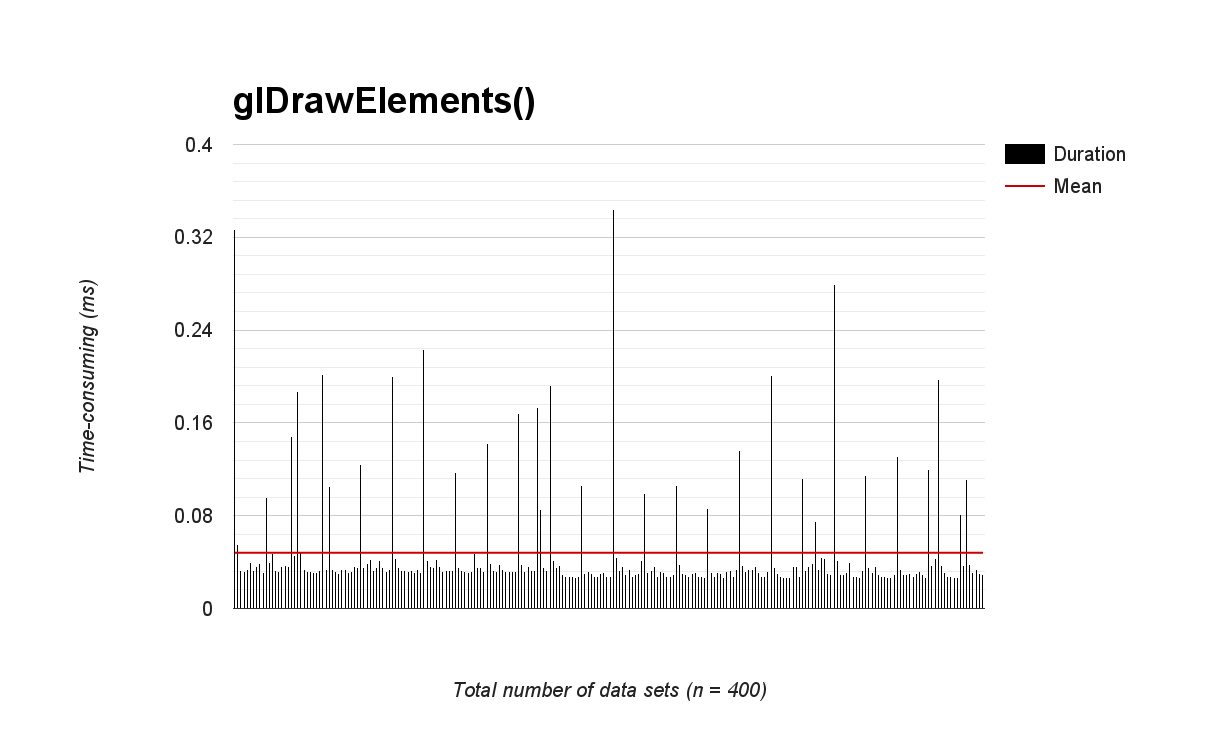
\includegraphics[width=\textwidth, keepaspectratio]{Figures/glDrawElements-performance.png}
	\decoRule
\end{figure}



%****************************************************************